\section{Discussion of Results}\label{sec:result}
    
\subsection{Evaluation Against Other Approaches}

\rt{This is a very long block of text, spanning multiple pages. Can you add some paragraph titles, summarizing the gist of each paragraph/finding?}

\begin{figure*}
    \centering
    \includegraphics[width=0.70\linewidth]{analysis/artefact/variation_approach/reduction_query_execution_time}
    % General caption
    \caption{
    Comparison of query execution time with the type index approach.
    The ratio represents how the execution time of each method compares to that of the type index. 
    A ratio greater than $1$ indicates a slower execution time (\textbf{lower is better}).
    The shape index approach performs similarly or better than the other methods, except in the case of S4.
    }
    \label{fig:compApproach}
\end{figure*}

Figure~\ref{fig:compApproach} shows that the shape index approach performs better or comparably to the state-of-the-art Solid Pod network traversal algorithms, for all query templates except S4.
Figure~\ref{fig:compApproachRaw} in the \hyperref[sec:appendix]{Appendix} presents the execution times of each method and Table~\ref{tab:statSignificanceStateOfTheArt} presents the statistical significance by query templates.
The shape index approach allows for answering queries from the S7 template, which was not possible by the other approaches, due to large amount of HTTP requests resulting in timeouts.
Queries can require as little as 13\% of the execution time (S1 being 7 times faster) of the type index.
The queries that perform the best are those in which the number of HTTP requests decreased the most, as can be inferred from the analysis of Table~\ref{tab:ratioUsefulResources}.
This table presents the average percentage of query-relevant resources per query template, derived from the where-provenance~\cite{buneman2001and} of the query results and the number of HTTP requests. 
%Table~\ref{tab:statSignificanceStateOfTheArt} presents an analysis of the statistical significance of the query template and its relation to the ratio of HTTP requests performed.
Queries from templates D6 and D7 show no reduction because they require nearly every document in the dataset to be processed by the engine, making our approach ineffective in these cases.
We notice that queries from template S4 with the shape index performed worse in every instance, with an increase in query execution time of up to 2.80 times.
This is further illustrated in Table~\ref{tab:ratioUsefulResources}, which shows that for these queries, the type index traversal algorithm achieves a ratio of query-relevant resources dereferenced of 100\% or 50\%, compared to only 6\% with the shape index approach.
The poor performance is due to the fact that the links acquired by the other approaches were selected based on reachability criteria that did not leverage the structural properties of the dataset, such as in the case of \texttt{Cmatch}~\cite{hartig2016walking}, a reachability criterion based on the structure of the query.
In contrast, the shape index approach always enforces the use of these properties, resulting in additional HTTP requests and increased processing time.
%It has to be highlighted that our formalization assumes that structural assumptions are always used and that the shape index, if present, will be part of the traversal, see section~\ref{sec:sourceSelection}.
However, those queries were already efficient, with the type index traversal approach completing in only about 0.30\% of the maximum allowed execution time.
Nonetheless, these results still highlight a category of queries and networks for which our approach is not well-suited.
Those results mostly validate \textbf{H1} however the shape index approach can drastically increase the execution time when the structural properties are not used.

\input{analysis/artefact/ratio_useful_resources/table_ratio_useful_resources_summary} 
\rt{When just looking at the table, it is not clear what this table shows. I recommend a slight tweak in the caption: "\textbf{The percentage of query-relevant resources}, which are low for most queries."}

To further our analysis, we compare three temporal metrics: the arrival time of the first results, the termination time, defined as the duration between the arrival of the last result and the end of query execution, and the waiting time, which we define as the accumulated time gaps exceeding one second between the reception of consecutive results.
We choose a 1 second threshold for waiting time based on research in responsive system design.
These waiting time guidelines are derived from the field of neuropsychology and are considered stable regardless of technological expectation for human users~\cite{uxtigersNeedSpeed, Nielsen1993}.
A waiting time below 0.1 seconds is perceived as instantaneous, a delay of up to 1 second preserves a seamless flow of thought, while delays exceeding 10 seconds tend to cause user attention to drift~\cite{Nielsen1993}.
We additionally computed the diefficiency metric in relation to time (\textit{dief@t})~\cite{Acosta2017}, at the previously mentioned time intervals: 0.1\,s, 1\,s, and the arrival time of the final result.
We did not choose 10\,s as the threshold, because queries that terminate complete in under 10\,s.
Tables~\ref{tab:dief} and \ref{tab:continuousPerf} in the \hyperref[sec:appendix]{Appendix} present the average results for the metrics presented above.

\begin{figure}
    \centering
    \includesvg[width=\linewidth]{analysis/artefact/continuous_performance/first_result}
    \caption{
    \textbf{The first result distribution by query template.}    
    The shape index approach tends to produce the first results earlier than the type index approach, particularly for queries where the shape index achieves shorter total execution times.}
    \label{fig:first_res}
\end{figure}

Figure~\ref{fig:first_res} presents the time of arrival of the first results for all query instances, grouped by query templates. 
The plot indicates that, for most queries, the shape index approach tends to produce results faster, as shown by distributions concentrated around lower first result arrival times.
Templates D1, D2, D5, and S1 exhibit the most significant improvements in first-result latency when using the shape index.
Surprisingly, although queries from templates D2 and D5 sometimes performed worse with the shape index approach, as shown in Figure~\ref{fig:compApproach}, they still produced the first result faster than with the type index approach.
This suggests that, although the shape index does not explicitly prioritize early result generation, the pruning it performs may implicitly favor faster first results arrival with some queries and networks. 
This implicit prioritization does not apply uniformly across all templates. 
For example, queries from template D3 exhibit faster execution times across most instances when using the shape index.
However, as shown in Figure \ref{fig:first_res}, the shape index also results in a higher mean and a longer tail for the time to first result.
This difference arises from the structure of the subwebs targeted by D3 queries.
In some cases, a result can be obtained from a document located one link away from the seed document.
The direct dereferencing using the type index approach can exploit this proximity, enabling early result generation.
In contrast, the shape index approach may delay first result production because it relies on discovering the shape index documents before exploring the rest of the subweb.

\begin{figure}
    \centering
    \includesvg[width=\linewidth]{analysis/artefact/continuous_performance/termination_time}
    \caption{
     \textbf{The termination time distribution by query template.}    
    With the exception of queries from templates D6 and D7, which have similar execution times, the shape index either maintains or improves query termination time.}
    \label{fig:termination_time}
\end{figure}

Figure~\ref{fig:termination_time} presents the termination times for the query execution instances, grouped by template. 
For queries where execution time improved and termination time was non-zero, such as those from templates D1, S1, and S5, the shape index approach significantly reduces termination time. 
This improvement aligns with the substantial increase in the percentage of query-relevant resources dereferenced when using the shape index, as shown in Table~\ref{tab:ratioUsefulResources}.
A long termination time generally indicates that, toward the end of execution, a large number of non-query-relevant resources are being dereferenced. 
Although Table~\ref{tab:ratioUsefulResources} does not show the temporal progression of this percentage it still give us information about the quantity of non-query-relevant resources being dereferenced.
For templates D5 and D6, the termination-time distributions for the shape index approach have a similar shape but exhibit a longer tail, particularly D6, which can take up to one second longer to terminate. 
In these cases, Table~\ref{tab:ratioUsefulResources} shows that the proportion of query-relevant resources dereferenced using the shape index is within $\pm$1\% of that obtained with the type index.
A similar situation is observed for template D3, although in this case the type index achieves a termination time of zero. 
The longer termination times for D5 and D6 may be attributed to the additional dereferencing of shape index documents. 
Notably, for template D6 in Figure~\ref{fig:compApproach}, an outlier query increases execution time by approximately a ratio of 1.2, which could explain the extended tail and the additional second of termination time.


\begin{figure}
    \centering
    \includesvg[width=\linewidth]{analysis/artefact/continuous_performance/waiting_time}
    \caption{
    \textbf{The waiting time distribution by query template.}    
    Except for queries from template D1, the shape index approach tends to either maintain or worsen the waiting time.}
    \label{fig:waiting_time}
\end{figure}

Figure~\ref{fig:waiting_time} presents the waiting time for the query instances, grouped by template. 
With the exception of queries from the D1 template, which show a decrease in waiting time, the shape index approach generally increases the waiting time for queries that experience a delay before producing results. 
This increase is likely due to the additional dereferencing of shape index documents that must occur before relevant results can be generated. 
Such dereferencing can introduce a gap before the first results appear, even when the total query execution time is reduced or remains unchanged.


\begin{figure}
    \centering
    \includesvg[width=\linewidth]{analysis/artefact/continuous_performance/dief_01}
    \caption{
    \textbf{The \textit{dief@0.1s} distribution by query template.}    
    At 0.1 second, the value is zero for every query template except S4. This is expected, as for all other templates the first result arrives after 0.1 seconds.}
    \label{fig:dief_01}
\end{figure}

\begin{figure}
    \centering
    \includesvg[width=\linewidth]{analysis/artefact/continuous_performance/dief_1}
    \caption{
    \textbf{The \textit{dief@1s} distribution by query template.}    
    At 1 second, the shape index approach shows a higher \textit{dief@1s} (\textbf{higher is better}), indicating that more results are obtained while maintaining a seamless flow of thought.}
    \label{fig:dief_1}
\end{figure}


\begin{figure}
    \centering
    \includesvg[width=\linewidth]{analysis/artefact/continuous_performance/dief_lr}
    \caption{
    \textbf{The \textit{dief@lr} distribution by query template.}    
    At the time of the last result, the shape index approach tends to exhibit a similar \textit{dief@t} (\textbf{higher is better}).}
    \label{fig:dief_lr}
\end{figure}

Figures~\ref{fig:dief_01}, \ref{fig:dief_1}, and~\ref{fig:dief_lr} show the \textit{dief@t} values measured at 0.1 seconds (\textit{dief@0.1s}), 1 second (\textit{dief@1s}), and at the time of the last result (\textit{dief@lr}).\footnote{\label{fn:dief_lt}This means that if, for a given query, the shape index approach produces the last result at 5~seconds and the type index at 5.10~seconds, then the \textit{dief@t} metric will be computed at 5.10~seconds.}  
The \textit{dief@0.1s} results show that, except for S4, no approach is able to produce instantaneous results, which aligns with the observations in Figure~\ref{fig:first_res}.  
Overall, this indicates that, with the current approaches and benchmark, producing instantaneous results is not feasible.
The \textit{dief@1s} results indicate that the shape index approach generally produces a higher number of early results, except for queries from templates S4 and S5.
This result is expected for S4 as the performance with the shape index is drastically reduced as shown in Figure~\ref{fig:compApproach} however with S5 it is less expected as it is a query template that perform better with the shape index.
It would be expected to see a performance improvement in terms of \textit{dief@t} at the last results for S5, however, the values are zero or close to zero.
This is because these queries produce only a single result, so \textit{dief@t} naturally tends toward 0 unless there is a very large difference in execution time between the two approaches.~\ref{fn:dief_lt}
These results suggest that, for fast early result arrival, the shape index approach tends to performs better.
This finding is particularly relevant in the context of social media applications, where it is often more important to obtain fast, relevant results to maintain interactivity than to retrieve complete results.  
The \textit{dief@lr} show a similar behavior but with lesser performance gain compare to \textit{dief@1s} (see Table~\ref{tab:dief} to compare the average values).

% calculate ratio

\subsection{Query-Shape Subsumption Evaluation} \label{sec:experimentAlgoSubsumption}

The empirical evaluation of the query-shape subsumption algorithm shows that its execution time with the more detailed shapes from our experiment is negligible, with a maximum execution time of 4.655 ms (0.0039\% of the timeout).
Table~\ref{tab:queryShapeContainmentEval} present these results.
This outcome is expected, as the algorithm has polynomial time complexity, and the shapes and queries in the experiments are small and not deeply nested.
This result validates \textbf{H2}.


\subsection{Evaluation of the Resilience of the approach}

The final part of the results analysis focuses on the resilience of the shape index approach.
In this analysis, we examine the impact of reducing the shape index information in the network and compare the results with a network in which all pods are exposed to detailed, complete shape indexes.
Figure~\ref{fig:adaptShapeIndex} presents three plots that illustrate the results of our evaluation of the approach's resilience.
The plot on the left shows the variation in the availability of shape indexes across the network. 
As expected, we observe that queries that performed better in Figure~\ref{fig:compApproach} tend to perform worse with reduced shape index information, while queries that performed poorly improved. 
%Queries that were unaffected by the shape index changes remain unaffected.


\begin{figure*}
    \centering
    \includegraphics[width=1\linewidth]{analysis/artefact/variation_shape_index_all/plot}
    \caption{
    Shape index approaches tend to perform less effectively with limited network information and comparatively better where the baseline shape index underperforms.
    A higher ratio indicates a longer query execution time compared to a network with complete shape index information (\textbf{lower is better}).
    %However, the utility of shape index information can vary depending on the specific queries and network characteristics.
    }
    \label{fig:adaptShapeIndex}
\end{figure*}


The plot in the middle shows the variation in the percentage of shape index entries using closed shapes.
The results here are more nuanced.
While there is a general trend for query evaluations with a lower percentage of closed shapes to behave similarly to the plot on the left, we also observe both performance gains for some query templates and a drastic performance loss for the queries of S1 when 80\% of the shape entries are closed.
The performance gain occurs because not every entry needs to be closed to prune the query irrelevant documents.
Entries mapped to an open shape are always considered relevant because the shape translates to a query fetching the whole KG.
If the subsumption check leads to the same conclusion, then, given a closed entry, the execution will be more expensive because 
when shapes are nested, the nested shapes need to be dereferenced to solve the query-shape subsumption algorithm.
For the queries of S1, with 80\% of closed shape entries, the performance lost was due to random chance, as the discriminatory entries were provided with open shapes in multiple instances when looking at the raw data.

The right plot shows the variation in the level of detail of the shapes by reducing their detail.
Since the shapes are closed in this experiment the level of detail was varied by changing the constraint of the object terms.
Most queries tend to perform similarly or better, with the exception of those of S1.
Upon analyzing the output of our query subsumption algorithm, we observe that the additional information to the shape provided in our base approach does not affect the algorithm's results.
However, in the baseline shape index experiment, the engine must dereference more shapes, potentially increasing execution time.
Queries of template S1 are the only ones where the added information can discriminate multiple parts of the datasets' domain leading to worse performane.
This indicates that in some situations, adding more information can be beneficial.
This sensitivity of the quantity of the information in the index also helps explaining the results for S1 queries in the middle plot. 
In that case, the engine still had to dereference shapes from each dataset, and the information available was likely insufficient to significantly discriminate between resources.

These results show that \textbf{H3} and \textbf{H4} are rejected: reducing information is not always detrimental to query execution.
It becomes detrimental only when the omitted information is critical for determining the query relevance of resources. 
Therefore, the outcome is dependent on both the query and the network. 
Moreover, the completeness of shape indexes has a smaller impact on performance than their presence or absence.
\textbf{H5} is accepted; it is possible to retain performance gains even in networks with reduced shape-index information.

\begin{figure*}[htbp]
    \centering
    % First figure
    \begin{minipage}[t]{0.45\linewidth}
        \centering
        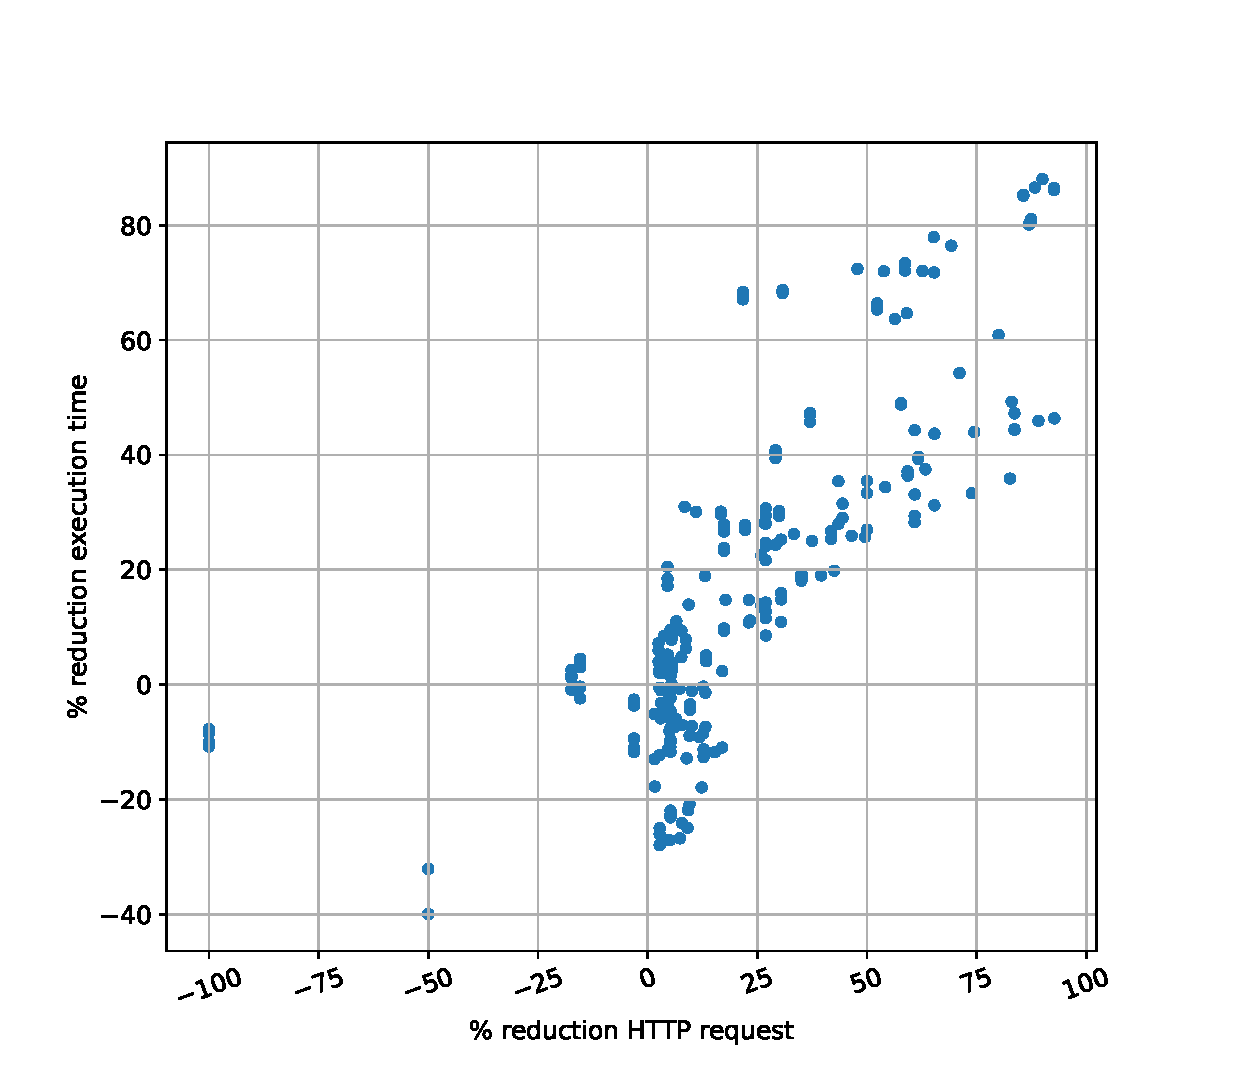
\includegraphics[width=\linewidth]{analysis/artefact/http_req_exec_time_relation/http_req_exec_time_cor_better}
        \label{fig:http_req_exec_time_cor_better}
    \end{minipage}
    \hspace{0.05\textwidth}
    % Second figure
    \begin{minipage}[t]{0.45\linewidth}
        \centering
        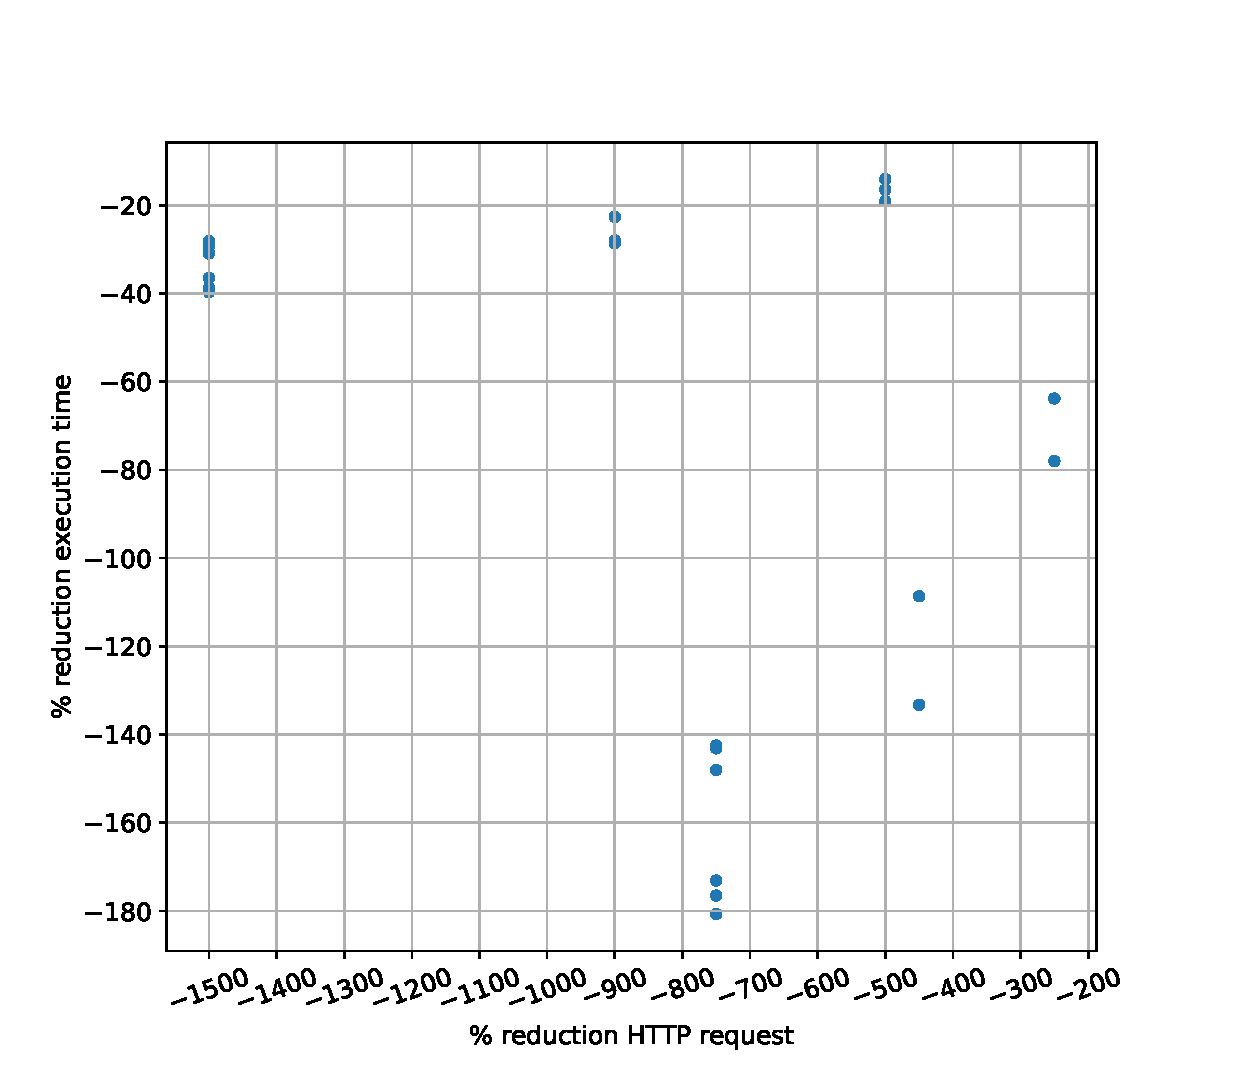
\includegraphics[width=\linewidth]{analysis/artefact/http_req_exec_time_relation/http_req_exec_time_cor_worse}
        \label{fig:http_req_exec_time_cor_worse}
    \end{minipage}

    % General caption
    \caption{
        The data show two regimes in the relation between the number of HTTP requests and the execution time, 
        we see a more linear correlation on the up figure than on the down figure.
        }
    \label{fig:http_req_exec_time_cor}
\end{figure*}

\subsection{Relationship Between HTTP Request and Query Execution Time}


To study the relationship between the number of HTTP request and the query execution time, the ratio of HTTP request of the different approaches and the ratio of query execution time was 
calculated in relation to the type index approach.
Figure~\ref{fig:http_req_exec_time_cor} presents our analysis.
The relationship between HTTP request and query execution time can be divided into two regimes.
In the first regime (left figure), where the shape index approach reduces the number of HTTP requests, we notice a positive linear correlation with a Pearson correlation coefficient (PCC) of 0.84 and a high statistical significance ($< 0.01$).
We can notice that toward the end, the curve appears to exhibit a more exponential behavior.
Evaluating an $R^2$ score with an exponential best fit curve we get a score of 0.72 and 0.71 for a linear curve.
Above a ratio of approximately 0.85 of HTTP requests, the shape index approach did not guarantee a reduction in query execution time.
There can be multiple explanations for this behavior.
First, the methods have some overhead due to the query-shape subsumption algorithm and the state retention of the pruning reachability criteria.
However, the query-shape subsumption algorithm execution time is negligeable for one execution and the state retentation has a polynomial time complexity, thus it should not have a high impact on the execution time.
Another explanation is the number of HTTP requests that are performed in parallel.
The LTQP version of Comunica performs 10 HTTP requests in parallel, thus, we would expect that with a low number and ratio of HTTP requests, the performance would remain largely unchanged or slightly worse, which is what can be observed in the curve.

In the second regime (right figure), the shape index increases the number of HTTP requests.
We notice a moderate positive linear correlation with a PCC of 0.44.
The overall correlation between reducing HTTP requests and query execution time is positively linear, with a moderate linear correlation with a PCC of 0.56 and a high statistical significance.
The correlation is more linear than exponential with $R^2$ scores respectively of 0.31 and 0.24, however due to the low score it is difficult to determine the nature of the distribution.

Explaining the two behavioral regimes observed in the data is challenging.
One possible explanation for the poorer performance of the shape index approach in certain cases could be the low number of samples.
However, we also observe that the relationship between the two variables differs significantly across the regimes.
In the first regime, the relationship is close to one-to-one, with a slope of approximately 0.91.
In contrast, the second regime shows a much flatter slope of around 0.08, suggesting that the ratio of HTTP requests has a weaker influence.
This disparity indicates that the explanation may be more complex than just a sample size issue.
The increased number of HTTP requests can be attributed to queries executed using the D6, D7, and S4 templates, with the S4 template causing the largest increase.
Queries from the S4 template typically require only 1 or 2 HTTP requests, so when running with 10 concurrent requests, the impact on performance is limited.
On the other hand, queries using the D6 and D7 templates, executed with the type index traversal algorithm, required 26, 23, and 129 HTTP requests.
This significantly higher number of HTTP requests explains why the increase in HTTP requests had a greater impact on query execution time.

These results partially validate \textbf{H6}, as a linear relationship is observed when there are a sufficient number of HTTP requests and a significant reduction ratio, taking concurrent requests into account.